\documentclass[a4paper,12pt]{article}
\usepackage{ctex} % 支持中文
\usepackage{amsmath, amssymb} % 数学公式
\usepackage{graphicx} % 图片插入
\usepackage{hyperref} % 超链接支持
\usepackage[margin=1in]{geometry} % 调整页边距
\usepackage{float} % 图片和表格定位
\usepackage{subfigure} % 子图包

% 设置页面的头部和底部
\usepackage{fancyhdr}
\pagestyle{fancy}
\fancyhf{}
\rhead{实验报告}
\lhead{\leftmark}
\rfoot{第 \thepage 页}

\title{作业1:从零开始构建三层神经网络分类器,实现图像分类}
\author{何益涵 \\ 20307110032}
\date{\today}

\begin{document}
\maketitle


\section{作业内容}
\subsection{任务描述}
手工搭建三层神经网络分类器,在数据集[Fashion-MNIST]上进行训练以实现图像分类。

\subsection{基本要求}
\begin{enumerate}
\item 本次作业要求自主实现反向传播,不允许使用pytorch,tensorflow等现成的支持自动微分的深度学习框架,可以使用numpy;
\item 最终提交的代码中应至少包含模型、训练、测试和参数查找四个部分,鼓励进行模块化设计;
\item 其中模型部分应允许自定义隐藏层大小、激活函数类型,支持通过反向传播计算给定损失的梯度;训练部分应实现SGD优化器、学习率下降、交叉熵损失和L2正则化,并能根据验证集指标自动保存最优的模型权重;参数查找环节要求调节学习率、隐藏层大小、正则化强度等超参数,观察并记录模型在不同超参数下的性能;测试部分需支持导入训练好的模型,输出在测试集上的分类准确率(Accuracy)。
\end{enumerate}

\section{项目地址}
本项目的地址为:

。。。。。

\section{Fashion-MNIST 数据集介绍}

Fashion-MNIST 是由德国在线时尚零售商 Zalando 的研究部门开发的一个数据集,专门用于测试机器学习算法在时尚领域的表现。该数据集旨在作为经典的 MNIST 数据集的现代替代品,因为后者通常被认为过于简单,不能充分代表现代计算机视觉任务的挑战。

Fashion-MNIST 包含来自 10 个类别的 70,000 张灰度图像,每个图像的分辨率为 28x28 像素。这些类别包括:T恤/上衣、裤子、套头衫、裙子、外套、凉鞋、衬衫、运动鞋、包以及短靴。数据集被分为两部分:60,000 张图像用于训练,10,000 张用于测试。

此数据集广泛用于教育和研究,涵盖了计算机视觉中的基本问题,如图像分类,并提供了一组相对现代和相关的图像。Fashion-MNIST 可以通过其 GitHub 页面或通过多种数据加载库(如 TensorFlow, PyTorch)下载,这些库提供了简便的接口直接加载数据。

为了方便使用者,数据集的维护者还提供了多种基线结果和代码,以帮助新用户快速开始他们的研究项目。更多信息和下载选项可以通过以下链接获得:\url{https://github.com/zalandoresearch/fashion-mnist}

\section{三层神经网络架构介绍}

本项目构建了一个不依赖任何外部框架的手写神经网络模型,它具有三个线性层和激活函数层。

\subsection{网络结构和初始化}
模型包括三个主要的线性层,每一层之间通过一个激活函数进行连接。第一层和第二层的激活函数默认为 ReLU,但可以通过参数替换为 Sigmoid 或 Tanh。所有线性层的权重通过 He 初始化来进行,这种初始化方法考虑到了前层神经元的数量,有助于在训练深层网络时保持激活函数的输出分布的方差一致。

\subsection{前向传播和后向传播}
在前向传播过程中,数据通过每一层的线性变换和激活函数,最终通过 softmax 函数输出预测的概率分布。后向传播利用损失函数关于输出的梯度,通过链式法则逐层计算并更新每一层的梯度。这一过程涉及到每个激活函数具体的梯度计算方法,以确保梯度的准确传递。

\subsection{参数更新和模型评估}
神经网络在后向传播后需要更新权重和偏置,通过梯度下降或其他优化算法逐步优化网络参数以减小预测误差。模型训练完毕后,可以通过评估模式关闭某些仅在训练阶段使用的特性(如 Dropout),以评估模型在未见数据上的表现。


\section{训练与测试方法}


\subsection{数据准备}
下载所需的数据集,进行必要的预处理操作。步骤包括标准化、归一化以及其他可能的数据清洗工作,以确保数据质量。之后,数据被分割为训练集和验证集,进一步组织成适合训练的批次。

\subsection{超参数调优}
在模型训练之前,需要对超参数进行细致的调整。这一过程涉及到多个参数,如学习率、隐藏层的规模以及正则化强度。为了简化调整过程,第二隐藏层的宽度被固定为第一隐藏层的一半,因此主要调节的是第一隐藏层的宽度和其他参数。通过一系列实验,记录下产生最佳验证效果的超参数组合。

\subsection{模型训练}
使用经过调优的最佳超参数组合,重新训练模型。此过程中,记录详细的训练历史,包括每个训练阶段的损失和准确率,以监控训练过程的进展和模型的性能。

\subsection{权重可视化}
为了更好地理解模型的内部工作机制,将对隐藏层的权重进行可视化。

\subsection{测试集评估}
最后,使用之前未见过的测试集对模型进行最终验证,确保模型在新的、独立的数据上也能表现出良好的预测能力。


\section{项目架构}
本项目包括以下主要文件:
\begin{enumerate}
    \item \texttt{model.py}:包含模型构造类、权重的保存与加载函数以及权重可视化函数。
    \item \texttt{data\_handling.py}:包含数据的下载与预处理函数。
    \item \texttt{training.py}:包含训练函数及训练过程的可视化函数。
    \item \texttt{testing.py}:包含对测试集进行实验的函数。
    \item \texttt{main\_notebook.ipynb}:包含实验的主要流程,超参数的微调环节也集成在此文件中。
\end{enumerate}



\section{模型训练结果}
\subsection{调参结果}

经过多次实验,最后一次实验的参数搜索范围定为:学习率(\texttt{lr}):\{0.00075,0.001, 0.00125\}、隐藏层大小(\texttt{hidden\_size}):\{512\}、权重衰减(\texttt{weight\_decay}):\{0,0.2, 0.4\}。以下是一些关键观察结果。

实验中发现,最优的参数配置是学习率为0.001,隐藏层大小为512,且不使用权重衰减(\texttt{weight\_decay=0})。在这个配置下,模型在验证集上的准确率达到了最高,为88.82\%。

权重衰减设置为0时,模型性能通常较好,表明在当前的数据集和网络结构下,权重衰减可能不是必需的,或者当前设置的权重衰减值过高。随着权重衰减的增加(例如0.2, 0.4),观察到验证集上的准确率有所下降,这表明较高的权重衰减可能导致过度正则化,进而影响模型的泛化能力。

较高的学习率(如0.00125)通常能带来更快的收敛,但有时可能会在后期导致准确率稳定或略有下降,这可能是由于学习率过高,在接近最优点时更新过于激烈。相反,较低的学习率(如0.00075)虽然在早期收敛较慢,但随着训练的进行,模型性能逐渐提高并保持了较高的稳定性。

在所有参数配置中,训练损失持续下降,显示出模型在有效学习训练数据的良好迹象。然而,验证损失在某些配置中在初期下降之后趋于平稳或轻微上升,这可能指示了过拟合的初步迹象,尤其是在没有权重衰减的情况下更为明显。

综上所述,最佳的模型配置不使用权重衰减,这可能表明对于当前的数据集和模型架构,简化模型(不使用正则化)足以达到良好的性能。对于这个具体案例,学习率为0.001时模型性能最佳,可能是因为它提供了速度与收敛质量的最佳平衡。

未来可能会在训练中尝试在更小的范围内细调学习率,以探索是否能进一步提升模型性能。此外,考虑实验不同的模型架构或更深的网络,以及实验轻微的权重衰减(如0.1以下),来看是否能在不牺牲准确率的情况下增强模型的泛化能力。


\subsection{训练与测试结果}
最优超参数的训练结果如下。可以看出模型的精度尚可,但是已经出现了轻微的过拟合。

\begin{figure}[H]
    \centering
    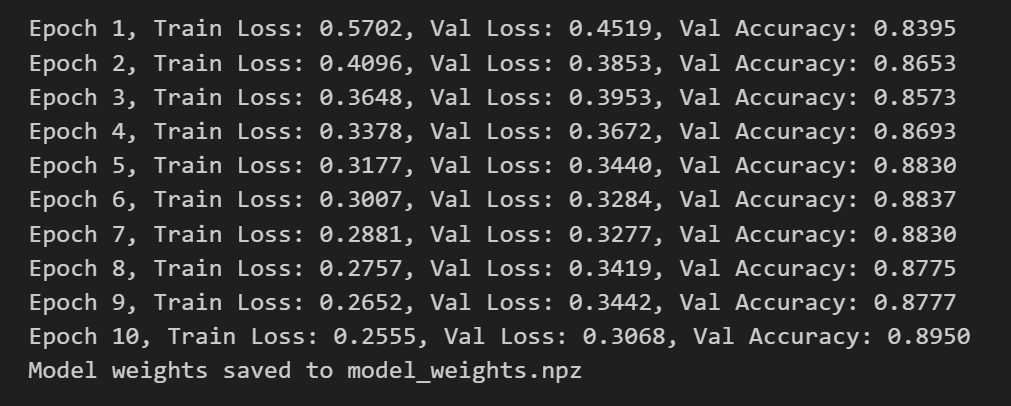
\includegraphics[width=0.9\textwidth]{train_stat.png}
    \caption{最优超参数训练数据}
    \label{fig:example}
\end{figure}

\begin{figure}[H]
    \centering
    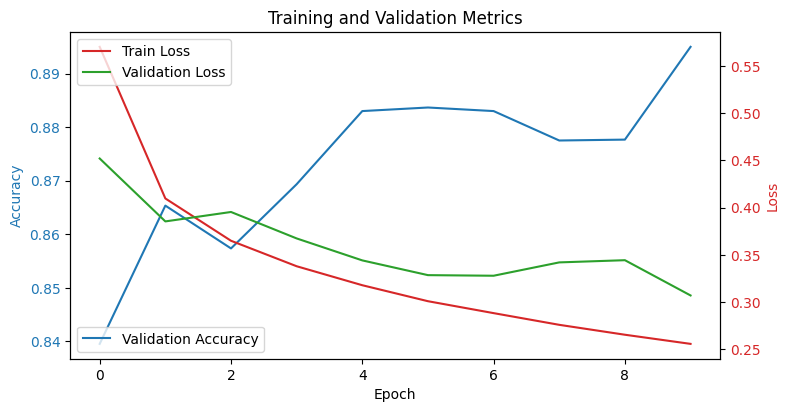
\includegraphics[width=1\textwidth]{train_graph.png}
    \caption{最优超参数训练示意图}
    \label{fig:example}
\end{figure}

最终,模型在测试集上的结果与在训练集和验证集上相似,精度为0.8846,说明模型的泛化能力是不错的。

\begin{figure}[H]
    \centering
    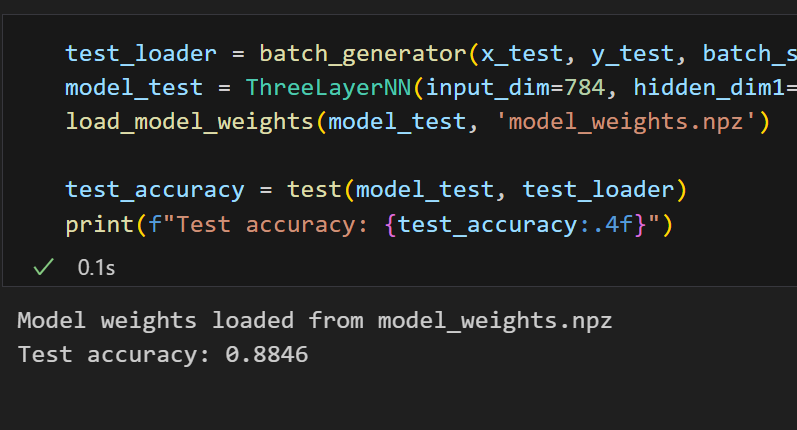
\includegraphics[width=1\textwidth]{test.png}
    \caption{测试集结果}
    \label{fig:example}
\end{figure}

\section{权重可视化}
以下是三个线性层的可视化结果。需要注意图中的序号是考虑了激活层的标号。

\subsection{前两层权重分析}
\begin{itemize}
    \item 权重分布相对均匀,没有明显的模式或结构,这可能意味着这一层的神经元没有形成对特定特征的强烈偏好。
    \item 权重值集中在较小的范围内,大多数位于 -0.1 到 0.1 之间,这表明激活函数的输出波动不大,导致后续层的输入相对稳定。
\end{itemize}

\begin{figure}[H]
    \centering
    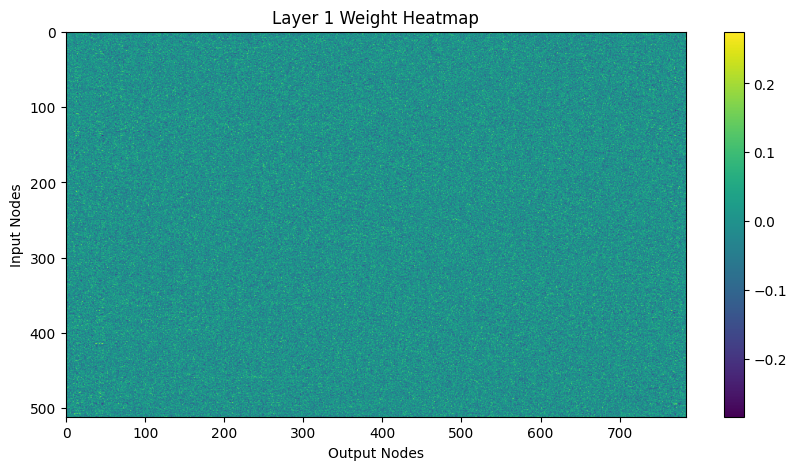
\includegraphics[width=1\textwidth]{layer1.png}
    \caption{第一层权重}
    \label{fig:example}
\end{figure}

\begin{figure}[H]
    \centering
    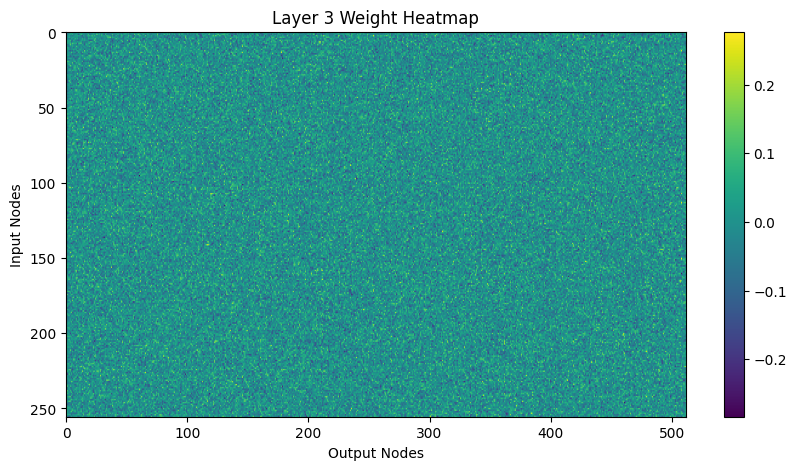
\includegraphics[width=1\textwidth]{layer2.png}
    \caption{第二层权重}
    \label{fig:example}
\end{figure}



\subsection{最终层权重分析}
\begin{itemize}
    \item 权重分布显示出明显的垂直条纹,表明某些输出节点与特定输入节点的连接强度更高,反映了网络捕捉到的重要特征。
    \item 权重数值范围较广,从 -0.6 到 0.4,可能意味着这一层在特征重组上作用更为激烈,以做出最终决策。
    \item 条纹中的亮暗对比可能指示某些特征在分类任务中的重要性,亮色代表强正权重,而暗色代表强负权重。
\end{itemize}

\begin{figure}[H]
    \centering
    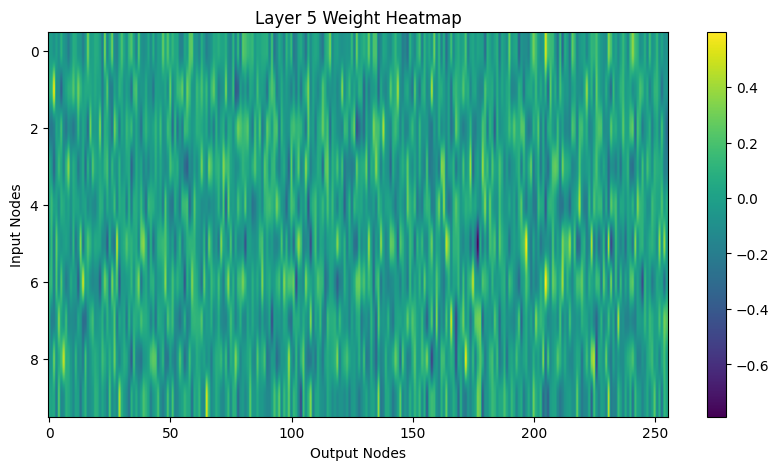
\includegraphics[width=1\textwidth]{layer3.png}
    \caption{第三层权重}
    \label{fig:example}
\end{figure}



\subsection{结论}
\begin{itemize}
    \item 前两层的权重可能表明其在语义上的作用不显著,处理的特征较为简单。
    \item 最终层的权重分化强烈,表明它在决策过程中扮演了关键角色,因为它是最终分类层。

\end{itemize}

\end{document}
